% JEL-Article.tex for AEA last revised 22 June 2011
\documentclass[JEL]{AEA}
\usepackage{hyperref}

% The mathtime package uses a Times font instead of Computer Modern.
% Uncomment the line below if you wish to use the mathtime package:
%\usepackage[cmbold]{mathtime}
% Note that miktex, by default, configures the mathtime package to use commercial fonts
% which you may not have. If you would like to use mathtime but you are seeing error
% messages about missing fonts (mtex.pfb, mtsy.pfb, or rmtmi.pfb) then please see
% the technical support document at http://www.aeaweb.org/templates/technical_support.pdf
% for instructions on fixing this problem.

% Note: you may use either harvard or natbib (but not both) to provide a wider
% variety of citation commands than latex supports natively. See below.

% Uncomment the next line to use the natbib package with bibtex 
\usepackage{natbib}
\usepackage{tikz}

% Uncomment the next line to use the harvard package with bibtex
%\usepackage[abbr]{harvard}

% This command determines the leading (vertical space between lines) in draft mode
% with 1.5 corresponding to "double" spacing.
\draftSpacing{1.5}

\begin{document}

\title{Congestion Pricing and Information: An Overview}
\shortTitle{Congestion Pricing and Information}
\author{Eric Tang\thanks{%
Stanford University; 450 Serra Mall, Stanford CA 94305; etang21@stanford.edu.
I am deeply grateful to Matthew Gentzkow for advising and guiding this directed reading. I thank Paul Milgrom for suggesting several recent papers on carpooling and congestion pricing.
}}
\date{\today}
\pubMonth{March}
\pubYear{2021}
\pubVolume{}
\pubIssue{}
\Keywords{congestion pricing, routing, Braess' paradox, Bayesian persuasion}

\begin{abstract}
As long as cars have been on the road, both commuters and economists have fretted about welfare losses due to traffic congestion. In this work, we survey the literature on congestion games, congestion pricing, and the design of routing information systems. Beginning with the seminal work of \cite{vickrey-1969}, economists' preferred remedy to congestion has typically been congestion pricing, the practice of levying tolls on commuters during peak commute hours. With the recent implementation of congestion pricing in cities such as London and Singapore, empirical work on the welfare effects of congestion pricing has grown. However, opponents of congestion pricing argue that poorer individuals disproportionately bear the burden congestion tolls. We review this theoretical and empirical literature on welfare and distributional effects of congestion pricing. Recent technological work has also stimulated work on the effects of navigation platforms and ridesharing. We discuss these advances, focusing on the effects of greater information for commuters facing congestion.
\end{abstract}

\maketitle

Traffic is a significant burden for commuters and economies; in the United States alone, the economic costs of traffic congestion have been estimated at around \$87 billion per year (\cite{fleming-2018}). With rapid urbanization continuing to create dense cities susceptible to traffic congestion (\cite{bryan-2020}), the costs of traffic congestion remain both a daily nuisance and a pressing problem for policymakers.

Beginning with \cite{vickrey-1969}, economists have typically proposed congestion pricing to reduce congestion. Under most congestion pricing models, commuters pay a variable toll for driving during peak travel times, or for traveling on highly-trafficked roads. Variations on this model have been implemented in several cities, including Stockholm (\cite{eliasson-2006}) and Singapore (\cite{olszweski-2005}), with notable impacts on average travel times.

However, congestion pricing has also been criticized as a potentiallly regressive tax. If poor individuals commute more often or have less schedule flexibility, the burden of congestion tolls will tend to fall more heavily on low-income commuters. Furthermore, the benefits of reduced congestion may largely accure to high-income individuals who have higher monetary valuations for their time. This has often galvanized political opposition to congestion pricing. Theoretical and empirical work analyzing the regressivity of congestion tolls, including \cite{arnott-1994}, \cite{small-1983} and \cite{eliasson-2006}, generally find that congestion tolls are regressive, but the ultimate effects of a policy depend on the mechanism used for redistributing a congestion tax's revenues.

Along with the classical literature on congestion models, new technologies such as traffic-aware route guidance and ridesharing platforms have motivated further interest in the field. Among this work, \cite{das-2017} and \cite{ostrovsky-2018} study how information provisioning and ridesharing technologies could be used to address congestion, and how these technologies might interact with standard congestion pricing models.


We survey the congestion pricing literature on welfare and distributional effects, as well as recent work motivated by information design approaches. Section \ref{early-congestion-models} introduces the classical models of congestion in road networks and congestion pricing. Sections \ref{welfare-effects} and \ref{distributional-effects} survey the welfare and distributional effects of congestion pricing, both from theoretical models and from city-specific evaluations of congestion pricing. Section \ref{information-provision} surveys more recent literature on the promises and risks of information provision in routing problems. Section \ref{carpooling-models} discusses models inspired by carpooling platforms and the possibility of autonomous vehicles. Finally, Section \ref{research-questions} suggests several open questions for future research in the field.

\section{Early Congestion Models}
\label{early-congestion-models}

A variety of theoretical work models the behavior of drivers facing congestion. The underlying structure of most of these models is similar, with several differences that authors can alter in their model. Congestion pricing models generally model a set of consumers and a set of routes, in which 

\begin{enumerate}
    \item Commuters choose between one of several source-to-destination routes.
    \item Commuters choose a departure time, given a desired arrival time.
    \item Commuters face a travel time that is a function of the number of other commuters on their route.
    \item Commuters' utilities are given as a function of travel time and arrival time.
\end{enumerate}

Typically, equilibrium concepts in these theoretical models are restricted to those outcomes where each agent is maximizing their utility while holding other commuters' actions fixed. Despite this basic structure, models vary widely in the details of each component. 

The classic congestion pricing model is that of \cite{vickrey-1969} with a single route and homogeneous consumers. Vickrey considers a model with commuters who have homogeneous valuations for time spent in traffic, and time spent at their destination before and after a desired arrival time. He considers a bottleneck model of congestion, in which a queue gradually accumulates along the route, then is reduced as time progresses and the cars leave. He then considers a variable toll, in which the crossing toll gradually increases as the typical hour of congestion approaches. Under this toll regimen, commuters are indifferent between paying the toll and the (previous) equilibrium in which they remained in traffic. Thus the net surplus is the revenues collected by the toll, with no change to commuters' net welfare. Later modeling work such as \cite{eliasson-2006}, deal with the critical issue of how to redistribute these toll revenues.

\cite{arnott-1994} extend Vickrey's model to heterogeneous consumers, who can vary along several dimensions. Among their extensions, consumers may vary by their desired arrival time, by their valuation of time spent traveling, and by the disutility incurred from late arrival. This heterogeneity is motivated by differences in commuters based on their incomes and type of work. In one example which Arnott et al. give, a manufacturing worker who must clock in at 8:00 am on the dot will likely have an inflexibile response to a congestion toll, whereas a manager with greater schedule flexibility may be able to avoid peak travel tolls. Furthermore, if the worker has a lower valuation for their time, they will likely enjoy fewer benefits of the congestion price than a manager who has a high valuation for their time. \cite{arnott-1994} analyze this model and its equity implications, which are discussed in a later section. Building on \cite{vickrey-1969}, they also model a simple redistribution of tolls in a lump-sum redistribution. 

The more recent work of \cite{das-2017} and \cite{ostrovsky-2018} both model road networks with multiple routes between sources and destinations. In these models, a key response of commuters to any congestion price is their ability to choose different routes to their desired destination. However, \cite{arnott-1990} models and argues that the efficiency gains of commuters shifting their travel \emph{times} is likely to dominate the effect of commuters shifting their travel \emph{routes}. As in the classical models, most of the recent work on information provision in commuting, such as \cite{das-2017} and \cite{acemoglu-2016} continue to focus on road networks with one source and one destination.

\section{Welfare Effects of Congestion Pricing}
\label{welfare-effects}

We now turn to the estimated welfare and distribution effects of congestion pricing. Along with the wealth of theoretical models on congestion, there is now a sizable body of empirical work, using measurements of commuter behavior in the real world. Several of these arise from cities which have implemented congestion pricing systems, such as Stockholm, Singapore, and London. Others, such as \cite{kreindler-2018}, measure interventions in cities that do not have widespread congestion pricing.

Estimating the welfare effects of proposed congestion prices typically requires estimates both of how the prices will change commuter behavior, and of commuters' valuations for travel time and arrival time parameters. \cite{kreindler-2018} collects a panel data set on the travel patterns of commuters in Bangalore, India who were randomly enrolled in one of several congestion pricing treatment groups. Kreindler uses this data principally to estimate commuters' valuations for time and their valuations of early arrival time. In a novel step, Kreindler then uses these estimates to estimate the optimal congestion pricing policy, as welll as the resulting change in commuter welfare. He finds that while the optimal congestion pricing policy significantly reduces travel times, its welfare gains are almost entirely offset by the disutility of commuters having to depart at times which they do not prefer.

\cite{kreindler-2018} studies two congestion pricing models in particular: a ``departure time" toll, which penalizes drivers who depart at peak hours, and an ``area congestion'' toll, which penalizes drivers who drive through a particular area (the congested city center). He then models commuters in the spirit of \cite{arnott-1994}, in which commuters select a route and a departure time, and their choices are guided by their valuations for time and by their scheduel flexibility. With this collected panel data, Kreindler uses a revealed-preference approach to estimate these structural parameters, then simulates the optimal congestion pricing policy as an equilibrium in which the marginal social cost for a consumer departing at a given time is exactly the toll they face.

Kreindler notes that besides being a novel revealed-preference approach to estimate commuters' actual preferences, his is one of relatively few studies on congestion pricing in the developing world. Both \cite{kreindler-2018} and \cite{bryan-2020} stress the need for further work on the specifics of congestion pricing in the developing world. In this setting, Kreindler's results suggest that congestion pricing may have negligible welfare impacts, resulting from the undesirable changes it induces in commuters' schedules.

Other empirical work on the effect of congestion prices in practice include \cite{olszweski-2005}, who study motorists' shift in commuting behavior after Singapore's introduction of its Electronic Road Pricing (ERP) system. Olszweski and Xie calibrate a model in which commuters may alter their route or departure times in order to avoid congestion tolls. They argue that their model explains the observed changes in congestion and departure times after the ERP's introduction. Olszweski and Xie find great heterogeneity in consumer elasticities with regards to congestion pricing, as first modeled in \cite{arnott-1994}. As a result, they adopt a similar model with several groups of consumers with differing elasticities for their departure times, and use data from before and after the congestion price's introduction to calibrate their model.

Under this model, Olszweksi and Xie find that elasticity on highways is higher than elasticity at the exact city cordon. This stands to reason, as commuters can generally take one of several alternate routes when they on highways far from their destination. They also find that departure times are less elastic in the morning than at other times of day, and that commuters generally prefer to move travel earlier than to postpone travel. These both have somewhat intuitive explanations, as a morning commuter likely must arrive at their workplace by a certain time, and faces harsher penalties for arriving late.

However, neither \cite{kreindler-2018} nor \cite{olszweski-2005} analyze the distributional effects of the congestion price imposed on commuters in Singapore or Bangalore with regards to income. We now turn to these distributional effects.

\section{Distributional Effects of Congestion Pricing}
\label{distributional-effects}

The question of congestion pricing's differential impact on different income groups is critical to analyze. In particular, if poorer individuals tend to have longer commutes and less schedule flexibility, they may pay the brunt of any congestion toll. Furthermore, as alluded to in \cite{arnott-1994}, if wealthy individuals have a higher valuation of their time, they will disproportionately benefit from the reduction in congestion. This potential regressivity of a congestion toll is often the issue around which political opposition to congestion pricing coalesces.

Indeed, in congestion pricing models, \cite{arnott-1994} found that congestion taxes were likely to be regressive, and surveyed a range of literature finding the same. In their own model, \cite{arnott-1994} find that the benefits of a welfare-maximizing congestion tax are likely to be higher for commuters with a higher valuation of their time (concretely, a higher valuation for early arrival and a higher cost of time spent traveling). If valuation of time rises with income, we then expect the toll to be regressive.

In a separate model, \cite{small-1983} also finds that a congestion tax without a mechanism for returning revenues is likely to disproportionately burden low-income groups, primarily due to their lower monetary valuation of time. Notably, this result still holds even though \cite{small-1983} model a public transit alternative in their model, which might be expected to reduce the burden on those commuters facing a congestion toll. However, \cite{small-1983} further models congestion tolls in tandem with one of three plans for redistributing toll revenues to individuals. They find that all individuals are better off if these tolls are redistributed in any of the three schemes. Under a uniform lump sum redistribution of revenues, the combined time savings and redistributed revenue benefits are proportionally higher for low-income groups. They also argue that under progressive redistribution policies, revenues from congestion prices could result in both a net monetary transfer from high-income to low-income commuters, along with a uniform time saving for all commuters.

\cite{eliasson-2006} model the distributional effects of the congestion pricing plan proposed in Stockholm, Sweden, which was eventually implemented. They also find that the most important factor determining whether a congestion tax is regressive or progressive is the use of revenues generated by the toll. In this case, they find that if the Stockholm congestion tax revenues are used to improve public transit, the proposed scheme is actually progressive. They also highlight the importance of modeling public transportation when determining the distributional effects of congestion pricing.

Eliasson and Mattsson first outline the conflicting reasons why a congestion tax might be regressive or progressive. Congestion pricing may be regressive because the wealthy have higher value of time, hence will disproportionately benefit from reduced congestion. Furthemore, the poor may pay more in congestion charges if they drive more often. On the other hand, in cities where autos are faster than public transit, the rich will disproportionately use cars and be affected by the tax. This may be true of "European" city layouts, for example.

The empirical modeling by Eliasson and Mattsson is particularly keen. They deploy several sample enumeration models to predict a commuter's origin and destination zone as a function of each route's travel costs, travel times, and the commuter's income. They use a specialized model of the changes in traffic times for the Stockholm congestion prices to determine these travel costs and travel times, then apply their sample enumeration models to determine predicted consumer charges and travel times before and after the change. These charges can be nicely separated into three categories: charges paid, change in charges due to route shifting, and time savings.

As to the effects of the proposal, wealthy Stockholm residents use their cars far more, hence pay more in tolls and also experience greater time savings. The magnitude of this difference is quite striking, with the authors concluding that "the richest third will pay four times more charges than the poorest third. Taking also time savings and changes in travel pattern into account, the richest third will lose around 2.5 times more than the poorest third from the direct effects of the charges" (618). They stress that the most critical issue in determining if the tax is regressive, however, is how the revenue collected from the congestion tolls are used. It is worth noting that their work is primarily based on a European model where public transit is widely available, and these results likely do not easily translate to other cities.

As most work in this domain finds that the distribution of revenues is the critical factor in determining whether a congestion price is progressive or regressive, more work on the effects of revenue redistribution is necessary. From a political economy perspective, it could be interesting to analyze what packages of revenue redistribution and congestion tolling would be amenable to a voter base. It may also be valuable to study how revenues from congestion prices are used in practice, and whether these differ from those which are proposed in the above works.

\section{Information Provision in Congestion Games}
\label{information-provision}

With the rise of platforms which can provide commuters with real-time information on traffic conditions, such as Waze and Google Maps, economic research on information in routing and congestion games has proliferated in the past several decades. Much of this work links to the broader fields of information economics and information design; for an overview, see \cite{bergemann-2019}. In the framework of \cite{bergemann-2019}, one could view routing guidance platforms as information designers with an informational advantage over commuters. Early work typically models the effects of information provision, while \cite{das-2017} explicitly design an information provision scheme according to the Bayesian Persusasion paradigm of \cite{kamenica-2011}. We focus here on work in which routing guidance can be used to reduce societal costs of travel time and congestion. With that said, it is not clear that companies which provide routing guidance share this same objective.

An early study of the effect of information on total congestion times is due to \cite{arnott-1991}, who studied an extension of the classical Vickrey model. In their model, commuters select both a time to depart as well as one of two routes to their destination, both of which have stochastic congestion levels. They find that if drivers receive perfect information about traffic conditions, total congestion is reduced, but if only incomplete information is provided, total congestion may increase. One intuitive explanation they offer for this is ``concentration": if commuters receive common information, they may align on the same choice of route, leading to increased driver concentration and congestion on that route. This finding contrasts somewhat with that of \cite{das-2017}, who demonstrate a scenario in which complete information provision offers no gains in net congestion time, while well-designed incomplete information provision can reduce total congestion. The comparison of these two models emphasizes the possible gains from carefully design information provision systems.

\cite{ben-akiva-1991} highlight a phenomenon related to concentration, which they term ``overreaction," wherein drivers who are provided with route information fail to anticipate the reaction of other drivers to that information. As a result of other drivers changing their routes simultaneously, the new route chosen may fail to be the actual best route for that driver. One would expect then to see oscillation in congestion and travel times between routes, as an abundance of drivers continually shift back and forth. \cite{ben-akiva-1991} note that this has been observed in simulations, but do not note empirical examples of overreaction. The authors also suggest addressing ``concentration" by potentially providing a range of route suggestions to users with the same source and destination, in their words, to ``take into account specific individual preferences to guide vehicles along different routes." It is not clear if modern routing guidance platforms such as Google Maps make an effort to avoid overreaction or concentration by suggesting different routes to commuters making the same commute simultaneously.

In a different vein, \cite{das-2017} apply the Bayesian Persuasion framework developed in \cite{kamenica-2011} to design an optimal information provision scheme for a routing guidance platform. They demonstrate that incomplete provision of information to commuters can reduce total congestion time, when compared to the equilibria under no information or complete information. They first model the network of Figure \ref{das-fig-1}, where commuters choose between two routes. One route has a stochastic travel time that is not a function of the number of commuters, and one route has a travel time that is a fixed function of the number of commuters. 

Under their model, an information designer can observe congestion times and send a signal to commuters as to which route to take, which does not provide full information yet still results in an improved outcome. Intuitively, when the route unaffected by congestion is better, the information designer always recommends that route. When the route unaffected by congestion is worse, the information designer still sometimes recommends that route, reducing the externalities imposed by drivers taking the route affected by congestion. The design is analogous to the leading example in \cite{kamenica-2011} of a prosecutor sending a signal to a judge under a set of Bayesian constraints. Das, Kamenica and Mirka also measure the gains from partial information provision against the "price of anarchy" benchmarks introduced in \cite{roughgarden-2002}.

\begin{center}
    \begin{figure}
        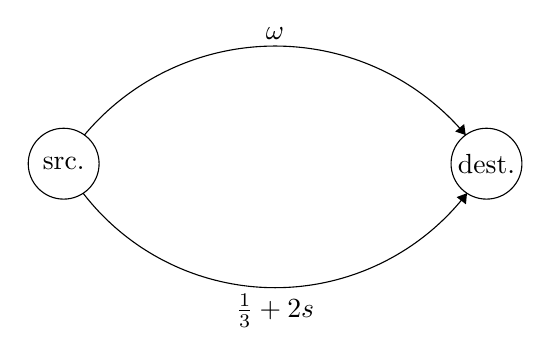
\begin{tikzpicture}[scale=0.15]
        \tikzstyle{every node}+=[inner sep=0pt]
        \draw [black] (21.6,-28.2) circle (3);
        \draw (21.6,-28.2) node {src.};
        \draw [black] (57.4,-28.2) circle (3);
        \draw (57.4,-28.2) node {dest.};
        \draw [black] (23.357,-25.772) arc (140.02578:39.97422:21.065);
        \fill [black] (55.64,-25.77) -- (55.51,-24.84) -- (54.75,-25.48);
        \draw (39.5,-17.74) node [above] {$\omega$};
        \draw [black] (55.75,-30.702) arc (-37.58626:-142.41374:20.507);
        \fill [black] (55.75,-30.7) -- (54.87,-31.03) -- (55.66,-31.64);
        \draw (39.5,-39.2) node [below] {$\frac{1}{3}+2s$};
        \end{tikzpicture}
    \caption{Road network studied in \cite{das-2017}. The lower route's travel time increases in the number of commuters $s$, while the upper route's travel time $\omega$ is stochastic and invariant to the number of commuters. }
    \label{das-fig-1}
    \end{figure}
\end{center}    


\cite{acemoglu-2016} study information in routing games in a different sense than \cite{das-2017}. In their context, commuters have distinct information sets representing which routes in the network they believe are accessible. Commuters gaining more information is equivalent to having an expanded information set about which routes are available to travel on. Similarly to previous models, the travel times along route segments are determined as functions of the commuters utilizing those segments. \cite{acemoglu-2016} then ask whether commuters being given more information can result in increased total travel times in equilibrium. This is an extension of the classic Braess' Paradox (in this case, adding a new route is akin to adding that route to all commuters' information sets), and \cite{acemoglu-2016} dub this an Informational Braess' Paradox.

To analyze equilibrium conditions, \cite{acemoglu-2016} first define a novel equilibrium concept, which they term Information Constrained Wardrop Equilibrium. In this equilibrium concept, commuters take the route in their information set with minimal congestion level, taking the level of congestion on each route as a given. The authors then fully characterize which routing networks are susceptible to the Informational Braess' Paradox. These are exactly those networks which are a series of linearly independent networks, where linearly independent networks are those in which each route has some edge which is not in any other route. They also prove results on the computational efficiency of determining whether a network is a series of linearly indpendent networks, and prove efficiency bounds on their equilibrium concept.

\cite{acemoglu-2016} also suggest several future directions for research, some of which are linked to those of other work on information in routing games. In a technical dimension, they note that their work only studies whether commuters with greater information provided to them are themselves harmed by more information; it is worth asking to what extent drivers without the given information also suffer greater congestion costs. Both \cite{das-2017} and \cite{acemoglu-2016} focus on networks with a single source and single destination, and suggest that further work on multiple sources and multiple destinations is necessary. Finally, they suggest a more empirical lens to determine whether informational Braess' paradoxes can be detected in the real world, and how likely such susceptible networks are to occur. This line of work is somewhat related to that of \cite{steinberg-1983}, who determined that the classic Braess' Paradox was about as likely as not to occur in general transportation networks. However, \cite{steinberg-1983} made no effort to identify such occurrences of Braess' Paradox in actual road layouts.

\section{Carpooling Models}
\label{carpooling-models}

Recent work has also been stimulated by questions of market design in a near future of autonomous vehicles. \cite{ostrovsky-2018} study the interaction of congestion pricing with carpooling, a practice which they argue will become more widespread with the emergence of autonomous vehicles.

\cite{ostrovsky-2018} first argue that carpooling and tolling are complementary ``technologies," which ought to be modelled in conjunction. As a guiding example, they consider the classic Vickrey model of congestion. Under this model, without tolls, agents have no individual incentive to carpool. With tolls and without carpooling, agents are indifferent between paying tolls and waiting in traffic, hence realize no surplus unless the toll revenues are redistributed to them. However, with tolls and carpooling, agents have an incentive to carpool, reducing total congestion on the road.

Ostrovsky and Schwartz next outline conditions that are sufficient for determining when an allocation of riders to routes maximizes social surplus. In their model, an outcome is an allocation of riders to (possibly shared) trips, each of which has a toll cost and a physical cost. Each rider has a valuation for each possible trip. The authors then introduce three conditions on these routing outcomes. They define \textit{budget-balanced} outcomes in the sense most common in the literature. \textit{Stable} outcomes borrow terminology from the literature on coalition formation and stable matchings: if no group of riders can organize an alternative trip that they would prefer, the outcome is stable. Finally, \textit{market-clearing} outcomes are those in which tolls are only imposed when needed: if a road segment is not at capacity, its toll is zero. This market-clearing condition provides a guide for how to set tolls to maximize social welfare. 

One main result of \cite{ostrovsky-2018} paper is that any feasible outcome which is budget-balanced, stable, and market-clearing must be a welfare-maximizing outcome among all feasible outcomes. With more work, they generalize these results to approximate outcomes, which they denote as ``quasi-feasible" outcomes, and address some of the technical issues caused by the discrete nature of the problem. Finally, they use their model to compare metrics of ``car utilization": they find that increasing the amount of time a car is on the road has relatively small savings compared to increasing the number of passengers in each car ride.

There are several policy implications of the work outlined above. First, when city planners model transit updates and tolls, it may be important to model these changes with carpooling considered. Second, their result on surplus-maximizing outcomes suggests that additive per-segment tolls, which do not vary by number of vehicle occupants, are sufficient to achieve optimal outcomes. Finally, their last result serves as further evidence for the power of carpooling to reduce total cost for commuters.

\section{Potential Research Questions}
\label{research-questions}

\begin{enumerate}

\item Opponents of congestion pricing often argue that such tolls are regressive, as poorer individuals often have longer commutes and will face tolls more often. Indeed, this has been a key issue in debates around congestion pricing in cities such as Singapore, London, and San Francisco. However, \cite{eliasson-2006} model a proposed congestion pricing plan in Stockholm, and find that the plan is actually progressive, as wealthy individuals tend to use their cars more often, and poorer individuals tend to use public transit. They attribute this finding to the robust public transportation system in Stockholm, and its traditionally ``European” city layout which favors public transit over automobiles. They and other authors caution against drawing the same conclusions in ``American” city layouts, where individuals tend to favor cars more often. \textbf{Can we more formally characterize what kinds of city layouts and public transit infrastructures result in congestion pricing being regressive? What implications does this have for city planners designing transit networks?}

\item \cite{kreindler-2018} notes that the model of commuter response to congestion prices, based on their valuation of time and their schedule flexibililty, takes only short-run factors into account. In the long-term, one might expect both commuters and businesses to adjust their behavior in the face of congestion pricing. For commuters, this could include increased work-from-home, shifting working hours, or moving to different locations. For businesses, one could imagine shifts in location, or offering employees different working hours. These shifts could negate any redistributive effects of a congestion toll, and particularly harm the poor: as an analogous example in the field of school choice, \cite{avery-2021} demonstrated that thanks to neighborhood relocation, improved school quality under a school choice scheme need not benefit low-income individuals. In this vein, \textbf{How do long-term relocation effects affect welfare estimates of congestion pricing policies? Will low-income individuals be most likely to relocate? How does this affect the distributional effects of any congestion pricing scheme?} I suspect that these effects may be relatively small, which could complicate the analysis.

\item \cite{small-1983}, \cite{arnott-1994} and \cite{eliasson-2006} all find that the critical policy issue determining whether a congestion toll is progressive or regressive is the manner in which its revenues are redistributed. This raises questions of what combined packages of redistribution and congestion tolls will be supported by municipal voters. It also raises concerns that revenues from congestion tolls may be captured after their implementation, altering a redistribution mechanism that may have initially been progressive. \textbf{How can we model voter support for plans that propose both a congestion toll and a concrete mechanism for spending the revenues of that toll? How are these revenues spent empirically, and when is the resulting package of tolls and spending progressive in practice?} 

\item \cite{arnott-1991} and \cite{ben-akiva-1991} describe the phenomena of ``concentration" and ``overreaction," when providing most commuters with route information can cause increases in congestion, or rapid oscillations in congestion levels between two routes. Intuitively, if a route guidance platform directs many commuters to the same route at the start of their journey, that route may no longer be optimal once commuters commit to the given route. \textbf{To what extent do routing guidance platforms attempt to mitigate concentration and overreaction, potentially by suggesting different routes to commuters with the same source and destination? What are the potential travel time gains from suggesting such distinct routes?}

\item Among the most general work studying when increased information provision harms commuters is that of \cite{acemoglu-2016}; they introduce the concept of an Informational Braess' Paradox (IBP) to describe the cases when making some subset of users aware of a route's existence worsens their equilibrium outcomes. However, Acemoglu et al.'s definition of IBP only asks whether the commuters who are provided with more information suffer worse outcomes, not whether other commuters suffer as well. These issues arise empirically as well: routing technologies such as Waze have been criticized for diverting traffic into neighborhoods where \href{https://www.washingtonpost.com/local/traffic-weary-homeowners-and-waze-are-at-war-again-guess-whos-winning/2016/06/05/c466df46-299d-11e6-b989-4e5479715b54_story.html}{residents resent the added congestion}. \textbf{Can we quantify the externalities imposed by providing information to some subset of commuters? That is, under what conditions does providing information to some commuters worsen equilibrium outcomes for other commuters?} This could take the form of defining a condition similar to that of IBP, then analyzing on what graphs that condition occurs.


\item \cite{das-2017} study the optimal provision of information to drivers in order to minimize net congestion in various road networks. Das, Kamenica and Mirka find that providing incomplete information to drivers can in fact reduce the societal costs of congestion. However, they note that if multiple firms can provide information to commuters, and commuters are free to switch between information providers, firms may have an incentive to provide (socially suboptimal) complete information. This is important in the real world, given that multiple platforms (e.g. Waze, Google, Apple) compete to provide drivers with congestion information, as \cite{ostrovsky-2018} allude to. \textbf{Can we model the behavior of such competitive firms who are providing information in congestion games? Does the presence of multiple firms always lead to full disclosure?} We note that for routing platforms who are perfectly informed about road conditions, the set of signals which firms can send is Blackwell-connected in the sense of \cite{gentzkow-2016}. As such, if all firms can send the same signals, there may be a straightforward characterization of what congestion information is disclosed in equilibrium.

\item \cite{das-2017} appear to be among the only authors to have applied ideas from Bayesian Persuasion to routing games. Their work studies a very specific case with one source, one destination, and a deterministic congestion function. This opens several doors for generalizing the model to incorporate more source and destination nodes, or stochastic congestion functions. One could even imagine modeling or simulating information provision on a road network from an existing city. \textbf{When is incomplete provision of congestion information still societally optimal under more complex transit models (e.g. multiple routes, multiple nodes, or stochastic congestion)? How does the improvement in congestion time change under these models?}


\end{enumerate}


% References here (manual or bibTeX). If you are using bibTeX, add your bib file 
% name in place of BibFile in the bibliography command.
% Remove or comment out the next two lines if you are not using bibtex.
\bibliographystyle{aea}
\bibliography{congestion}

% The appendix command is issued once, prior to all appendices, if any.
% \appendix

% \section{Mathematical Appendix}

\end{document}

